
\section{Modellierungstruktur}
\subsection{Modellierung des Hochwasserrisikos}
In diesem Abschnitt wird bei der Modellierung des Hochwasserrisikos die grundlegende Quantifizierung des physischen Risikos erläutert.
\subsubsection{Schadensfunktion}
Wie bereits in Abschnitt \ref{sec:tief} erwähnt, hängen die Schäden durch Überschwemmungen von der Wassertiefe ab. In diesem Abschnitt wird erklärt, wie diese Abhängigkeit konkret besteht.
Sobald verschiedene Flutwassertiefen ermittelt sind, wird eine spezifische Schadensfunktion für Wohnimmobilien \acs{RRE} entwickelt. Diese basiert auf der Methodik des Gemeinsamen Forschungszentrums \acs{JRC} der Europäischen Union \parencite{huizinga2017global}.

Da die Studie von \textcite{huizinga2007flood} unveröffentlicht ist, können die Daten nur aus den Diagrammen zur Schadensberechnung pro Quadratmeter und Schadensfaktor für verschiedene Regionen entnommen werden.

Abbildung \ref{fig:damage_curve1} und \ref{fig:damage_curve2} präsentieren zwei Grafiken, die die Schadenshöhe pro Quadratmeter und den Schadensfaktor für unterschiedliche europäische Regionen veranschaulichen.

\begin{figure}[H]
    \centering
    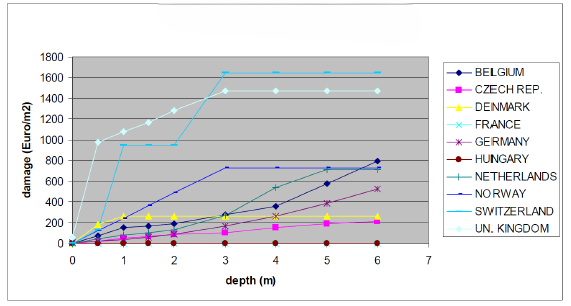
\includegraphics[width=0.8\textwidth]{figures/RREdamagem2.png}
    \caption{Schaden pro Quadratmeter in verschiedenen Regionen Europas. Quelle: J. Huizinga und al., 2017}
    \label{fig:damage_curve1}
\end{figure}

\begin{figure}[H]
    \centering
    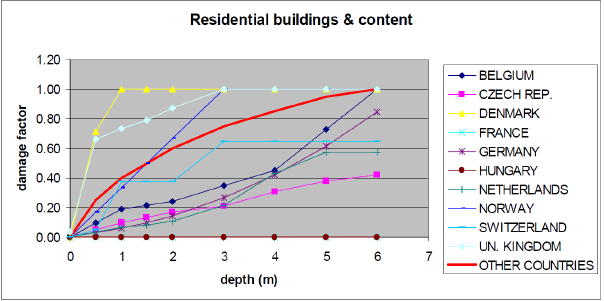
\includegraphics[width=0.8\textwidth]{figures/RREdamage.png}
    \caption{Schadensfaktor für Wohnimmobilien in verschiedenen Regionen Europas. Quelle: J. Huizinga und al., 2017}
    \label{fig:damage_curve2}
\end{figure}
\subsubsection{Berechnung von Hochwasserschäden}
Gemäß der Definition von der \textcite{undro1979,} ergibt sich das Risiko aus drei Komponenten: Gefährdungswahrscheinlichkeit,  den betroffenen Elemente (Exposition) und Vulnerabilität. \parencite{coburn1991vulnerability}. Dies kann vereinfacht ausgedrückt werden als:

\begin{equation}
    \text{Physisches Risiko} = \text{Gefährdungswahrscheinlichkeit} \times \text{Exposition} \times \text{Vulnerabilität}
\end{equation}

Um eine genauere Analyse der einzelnen Immobilienschäden zu ermöglichen, wird eine detailliertere Schadensformel \parencite{vanweddingen2023physicalrisk} benutzt:
\begin{equation}
    Immobilienschaden_{i,j} = E_j \times d(I_{i,j}|v_j)
    \label{eq:schaden}
\end{equation}
Wobei:
\begin{itemize}
    \item i das spezifische Ereignis bezeichnet
    \item $E_j$ den Wert der einzelnen Immobilie am Standort j repräsentiert
    \item $d$ die spezifische Schadensfunktion darstellt
    \item $I_{i,j}$ die lokale Intensität des Ereignisses i am Standort j ist
    \item $v_j$ die spezifische Vulnerabilität der einzelnen Immobilie am Standort j bezeichnet
\end{itemize}

Formel \ref{eq:schaden} berücksichtigt die Gefährdungswahrscheinlichkeit nicht, da sie den Schaden für ein einzelnes Ereignis berechnet. Für den erwarteten jährlichen Immobilienschaden wird die jährliche Überschreitungswahrscheinlichkeit aus Kapitel \ref{sec:EPC} benötigt und wird nachfolgend berechnet:
\begin{equation}
    EAI_j = \sum_i Immobilienschaden_{i,j} \times p(I_{i,j})
    \label{eq:EAI}
\end{equation}
Hierbei steht \acs{EAI} für den erwarteten jährlichen Schaden, und \( p(I_{i,j}) \) ist die Eintrittswahrscheinlichkeit des Ereignisses \( i \) mit der Intensität \( I_{i,j} \) am Standort \( j \).
Auf Grundlage der Formel \ref{eq:EAI} wird der erwartete Einfluss \acs{EI}, über die Kreditlaufzeit wie folgt berechnet:
\begin{equation}
    EI(j) = EAI(j) \times T
\end{equation}
Dabei ist \( EI(j) \) der gesamte erwartete Schaden über die Kreditlaufzeit \( T \).

Die Auswirkungen auf den Immobilienwert nach einem Schaden werden wie folgt berechnet:
\begin{equation}
    \text{Neuer Immobilienwert} = \text{Ursprünglicher Immobilienwert} - \text{Schaden}
\end{equation}

Zur Bestimmung der neuen Beleihungsquote \ac{LtV} auf Basis des angepassten Immobilienwertes gilt:
\begin{equation}
    \text{Neue LtV} = \frac{\text{Darlehenbetrag}}{\text{Neuer Immobilienwert}}
\end{equation}

Die risikogewichteten Aktiva \acs{RWA}, abhängig von der Beleihungsquote, berechnen sich folgendermaßen:
\begin{equation}
    RWA = \text{Darlehenbetrag} \times \text{Risikogewicht}
\end{equation}
Das Risikogewicht wird anhand der Beleihungsquote ermittelt.

Zum Schluss lässt sich die prozentuale Änderung der \acs{RWA} mit dieser Formel bestimmen:
\begin{equation}
    \% \text{Änderung RWA} = \frac{\text{Neue RWA}}{\text{Ursprüngliche RWA}} - 1
\end{equation}
